\documentclass[conference]{IEEEtran}

\usepackage{cite}
\usepackage{amsmath,amssymb,amsfonts}
\usepackage{graphicx}
\usepackage{textcomp}
\usepackage{xcolor}
\usepackage{booktabs}
\usepackage{multirow}
\usepackage{url}

\graphicspath{{../figures/}{../checkpoints/baseline_v2/}}

\begin{document}

\title{Robust Contactless Palmprint Verification with Deep Metric Learning:\\Checkpoint 1 --- Data Foundation \& Initial Modeling}

\author{
\IEEEauthorblockN{Huy Ong}
\IEEEauthorblockA{CS 228 -- Biometric Security\\Spring 2026}
}

\maketitle

\begin{abstract}
Contactless palmprint verification offers a hygienic and user-friendly biometric modality, but real-world capture variations can severely degrade system performance. This checkpoint report introduces our verification system built on the PolyU--IITD contactless palmprint dataset (611 subjects, 12,220 images) with a strict subject-disjoint evaluation protocol. We describe the data engineering pipeline, present exploratory data analysis, and detail our initial model architecture---ResNet18 with ArcFace angular margin loss. Training convergence analysis shows the model reaches stable performance by epoch 32, with validation EER of 1.13\%. Full test-set evaluation is deferred to Checkpoint~2.
\end{abstract}

% ============================================================
\section{Problem Statement}

Contactless palmprint verification is an emerging biometric modality that captures palm images without physical contact, improving hygiene and user acceptance compared to fingerprint sensors. Palmprints contain rich discriminative features---principal lines, wrinkles, and texture patterns---that remain stable over time, making them well-suited for identity verification~\cite{zhong2019palmprint, zhang2003palmcode}.

However, contactless capture introduces challenges absent in contact-based systems. Variations in hand pose, sensor distance, ambient lighting, motion blur, and compression artifacts all affect image quality. A practical verification system must not only achieve high accuracy on clean images but also degrade gracefully under these real-world conditions. When performance degrades, both security (increased false accepts) and usability (increased false rejects) are compromised.

This project addresses the question: \textit{How robust is a deep learning-based palmprint verification system to common real-world capture variations, and which factors pose the greatest risk to deployment?}

\subsection{Project Objectives}

\begin{enumerate}
    \item Train a deep metric learning model for palmprint verification with subject-disjoint evaluation.
    \item Establish baseline performance on clean data using standard biometric metrics (EER, FAR/FRR).
    \item Benchmark robustness under systematic image corruptions spanning noise, blur, geometric, and compression categories.
    \item Identify the most damaging degradation factors to guide future mitigation strategies.
\end{enumerate}

% ============================================================
\section{Data Engineering}

\subsection{Dataset}

We use the \textbf{PolyU--IITD Contactless Palmprint Database v3.0}~\cite{polyu}, comprising 611 subjects with 20 images each (10 left hand + 10 right hand), totaling 12,220 images. All images are 128$\times$128 grayscale ROI-cropped palmprint regions.

\subsection{Preprocessing Pipeline}

Each grayscale image is converted to 3-channel RGB for compatibility with ImageNet-pretrained backbones. Images are normalized using ImageNet channel statistics ($\mu = [0.485, 0.456, 0.406]$, $\sigma = [0.229, 0.224, 0.225]$). During training, we apply data augmentation including random cropping, horizontal flipping, rotation ($\pm$15\textdegree), color jitter, Gaussian blur, and random erasing to improve generalization.

\subsection{Subject-Disjoint Splits}

To prevent identity leakage, we use subject-disjoint splits where no subject appears in more than one partition. Each (subject, hand) combination is treated as a unique class, doubling the effective number of identities:

\begin{table}[h]
\centering
\caption{Dataset splits with subject-disjoint protocol.}
\label{tab:splits}
\begin{tabular}{lccc}
\toprule
\textbf{Split} & \textbf{Subjects} & \textbf{Images} & \textbf{Classes} \\
\midrule
Train      & 427 (70\%) & 8,540  & 854 \\
Validation & 61 (10\%)  & 1,220  & 122 \\
Test       & 123 (20\%) & 2,460  & 246 \\
\bottomrule
\end{tabular}
\end{table}

A quality audit identified 4 empty placeholder subjects (H\_ID608--611) in the original dataset; these were excluded from all splits.

% ============================================================
\section{Exploratory Data Analysis}

\subsection{Class Balance}

The dataset is perfectly balanced by design: each subject contributes exactly 10 images per hand, yielding uniform class sizes across all splits. This eliminates class imbalance as a confound in our evaluation. With 854 training classes each containing 10 samples, the model receives consistent supervision across identities.

\subsection{Sample Visualization}

The 128$\times$128 ROI-cropped images capture the central palm region containing principal lines, wrinkles, and texture patterns. Visual inspection confirms consistent quality across subjects, with clear visibility of discriminative features. Inter-subject variation in line patterns provides the basis for identity discrimination, while intra-subject consistency (across the 10 captures per hand) supports reliable matching.

\subsection{Corruption Types Overview}

To motivate our planned robustness evaluation, we preview the 9 corruption types that will be applied at 5 severity levels each. Fig.~\ref{fig:corruptions} illustrates these corruptions at severity level 3, spanning noise (Gaussian), blur (Gaussian, motion), geometric (rotation, scale), photometric (brightness, contrast), compression (JPEG), and occlusion categories. These corruptions model real-world capture degradations that a deployed system would encounter.

\begin{figure}[t]
\centering
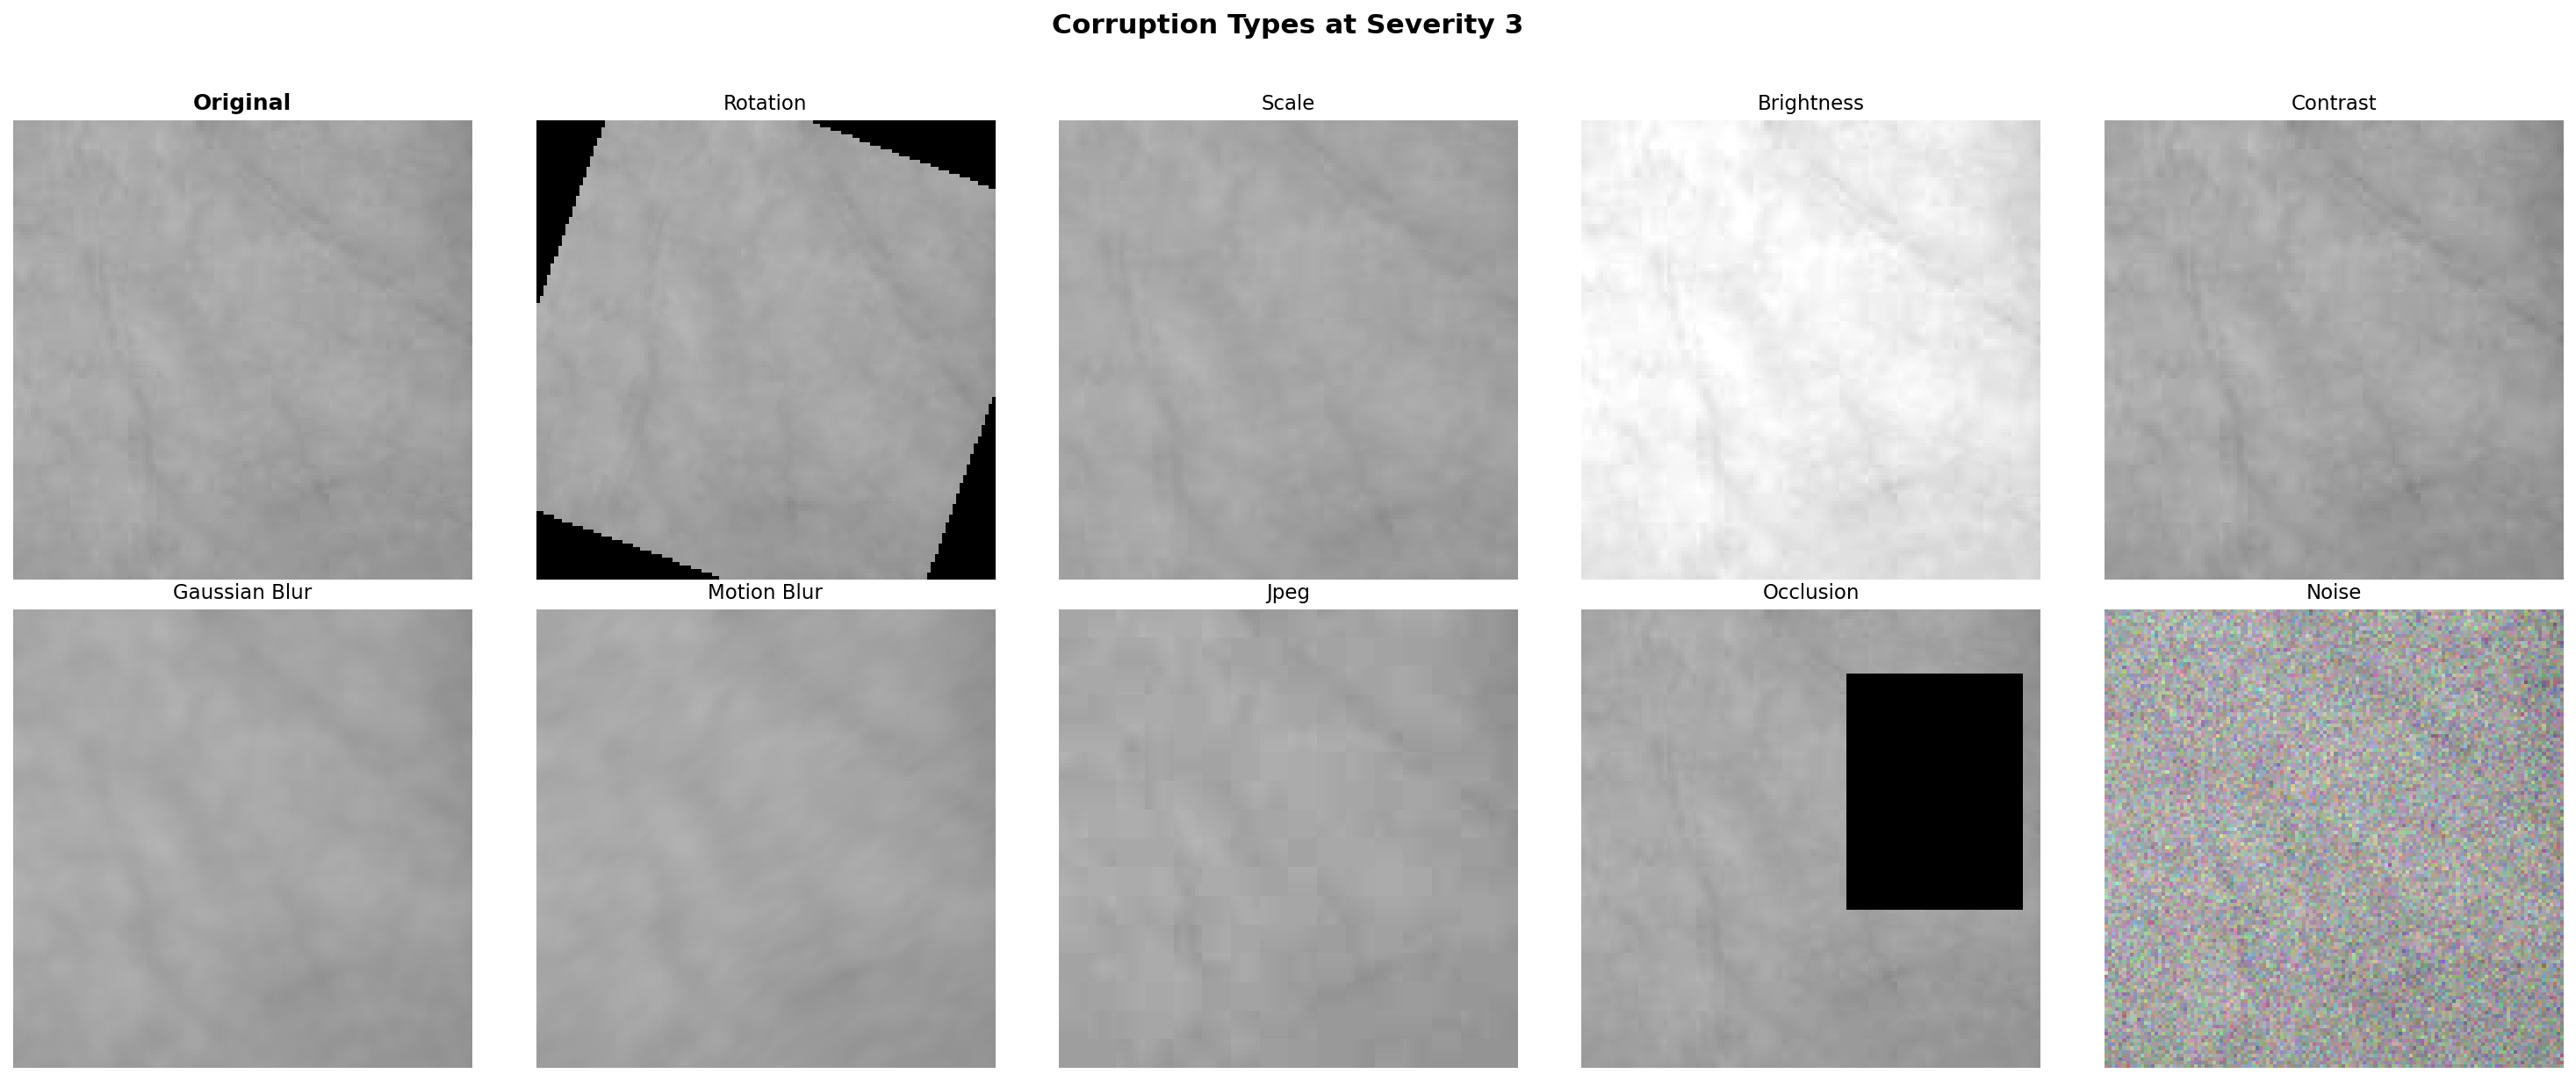
\includegraphics[width=\columnwidth]{corruption_samples.png}
\caption{Original palmprint image and 9 corruption types at severity level 3. Top row: Original, Rotation, Scale, Brightness, Contrast. Bottom row: Gaussian Blur, Motion Blur, JPEG, Occlusion, Noise.}
\label{fig:corruptions}
\end{figure}

% ============================================================
\section{Baseline Architecture and Training}

\subsection{Architecture}

Our model uses a two-stage architecture with approximately 12M parameters:

\begin{enumerate}
    \item \textbf{Backbone:} ResNet18~\cite{he2016deep} pretrained on ImageNet, with the final fully-connected layer replaced by an identity mapping, yielding 512-D feature vectors.
    \item \textbf{Projection Head:} A two-layer MLP ($512 \rightarrow 512 \rightarrow 256$) with batch normalization and ReLU, producing L2-normalized 256-D embeddings on the unit hypersphere.
\end{enumerate}

During training, an ArcFace~\cite{deng2019arcface} classification head computes $\text{logit}_j = s \cdot \cos(\theta_j + m \cdot \mathbb{1}[j = y])$ with scale $s = 30$ and angular margin $m = 0.3$. The ArcFace head is discarded at inference; only the embedder is used for verification via cosine similarity.

\subsection{Training Configuration}

The model is trained with AdamW (lr = $3 \times 10^{-4}$, weight decay = $10^{-3}$) and a cosine learning rate schedule for 50 epochs with early stopping. The best checkpoint is selected based on validation EER.

\subsection{Training Convergence}

Fig.~\ref{fig:training} shows the training convergence over 42 epochs (early stopping triggered). Key observations:
\begin{itemize}
    \item Training loss decreases from 8.3 to 1.5, indicating effective optimization.
    \item Training accuracy rises to 96\%, confirming the model learns to discriminate among 854 identities.
    \item Validation EER reaches a minimum of 1.13\% at epoch 32, which is selected as the best checkpoint.
\end{itemize}

The smooth convergence and low validation EER suggest the model has learned a discriminative embedding space. Full test-set evaluation with verification pair generation and robustness benchmarking will be presented in Checkpoint~2.

\begin{figure}[t]
\centering
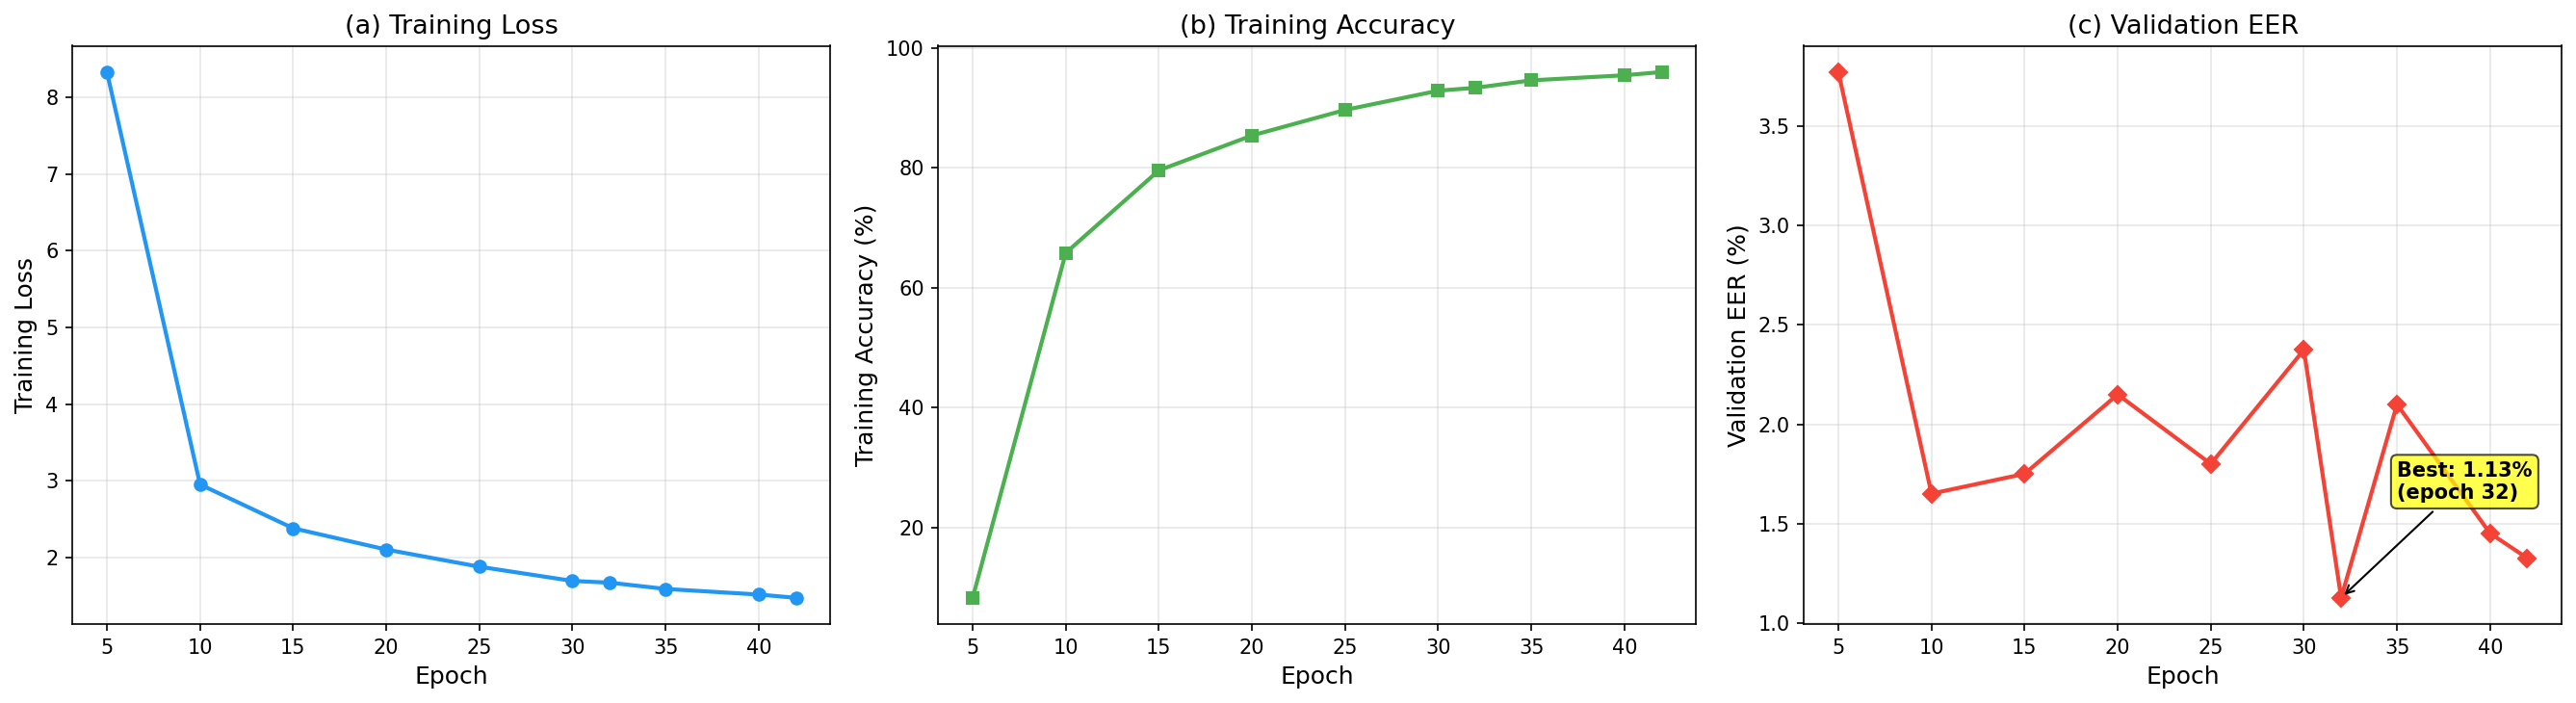
\includegraphics[width=\columnwidth]{training_curves.png}
\caption{Training convergence: (a) loss decreases from 8.3 to 1.5, (b) accuracy rises to 96\%, (c) validation EER reaches minimum 1.13\% at epoch 32.}
\label{fig:training}
\end{figure}

% ============================================================
\section{Code Repository}

The complete source code is available at: \texttt{https://github.com/onggiahuy97/cs228-palmprint}.

\medskip
\noindent\textbf{Repository structure:}
\begin{itemize}
    \item \texttt{src/} -- Training, evaluation, and data loading scripts
    \item \texttt{splits/} -- Subject-disjoint split definitions (JSON)
    \item \texttt{figures/} -- Generated plots and visualizations
    \item \texttt{checkpoints/} -- Model weights
    \item \texttt{requirements.txt} -- Python dependencies
    \item \texttt{README.md} -- Setup and usage instructions
\end{itemize}

\noindent\textbf{Key files:}
\begin{itemize}
    \item \texttt{src/train.py} -- Training loop with ArcFace loss and early stopping
    \item \texttt{src/dataset.py} -- Dataset class with augmentation pipeline
    \item \texttt{src/model.py} -- ResNet18 backbone + projection head
    \item \texttt{src/create\_splits.py} -- Subject-disjoint split generation
\end{itemize}

% ============================================================
\bibliographystyle{IEEEtran}
\begin{thebibliography}{5}

\bibitem{polyu}
PolyU--IITD Contactless Palmprint Database v3.0, The Hong Kong Polytechnic University.

\bibitem{deng2019arcface}
J.~Deng, J.~Guo, N.~Xue, and S.~Zafeiriou, ``ArcFace: Additive angular margin loss for deep face recognition,'' in \textit{Proc. IEEE/CVF CVPR}, 2019, pp.~4690--4699.

\bibitem{he2016deep}
K.~He, X.~Zhang, S.~Ren, and J.~Sun, ``Deep residual learning for image recognition,'' in \textit{Proc. IEEE CVPR}, 2016, pp.~770--778.

\bibitem{zhong2019palmprint}
D.~Zhong, X.~Du, and K.~Zhong, ``Decade progress of palmprint recognition: A brief survey,'' \textit{Neurocomputing}, vol.~328, pp.~16--28, 2019.

\bibitem{zhang2003palmcode}
D.~Zhang, W.-K.~Kong, J.~You, and M.~Wong, ``Online palmprint identification,'' \textit{IEEE Trans. Pattern Anal. Mach. Intell.}, vol.~25, no.~9, pp.~1041--1050, 2003.

\end{thebibliography}

\end{document}
